\section{Background}


Since the dawn of the 21st century, the era of 'Big Data' is shaping the way people live, learn and entertain. 
The need to handle the exponentially generated and accumulated data from varied sources like mobile devices, mechanical sensors, financial transactions,
satellite imaging makes the task of data managing gets much more challenging
day after day. 
With the usage of digital gadgets and industrial machinery presents a rapid increase, the amount of data generated reaches an astonishing level that is far higher than ever in history. 
According to a fact sheet organized by Mark Mulcahy \cite{factsheet} from Waterford Technologies, 2.7 Zetabytes of data exist in the digital world today, in which social media platforms like Facebook stores, accesses, and analyzes 30+ Petabytes of user generated data; search engines like Google was processing 20,000 terabytes of data (20 petabytes) a day; retail industries like Walmart handles more than 1 million customer transactions every hour. 
Besides the volume of data, the collected raw data are in a wide range of
forms, most are unstructured, like images, videos, audios, etc. YouTube users upload 48 hours of new video every minute of the day \cite{youtube}. And according to Twitter's own research in early 2012 \cite{factsheet}, it sees roughly 175 million tweets every day, and has more than 465 million accounts. The rampant usage of social media such as Twitter, Facebook, etc. is majorly responsible for such a severe data proliferation for the total size of the
data, contributed by the social media itself is approximately 90\% of the total data available \cite{DBLP:journals/corr/Sharma15b}.  \\

In the
whole data processing pipeline, starting from data integrating and
storing, it's already a quite essential part. Since the consistency,
accessibility, velocity of data inserting and retrieving might make a
huge difference to the following data manipulation tasks, especially in
fields like finance, social networks, etc. Thus making an optimal choice
of the right database for different data format, different data volume,
different business focus like whether velocity or consistency is more
important for the client's perspective.

\begin{figure}[H]
	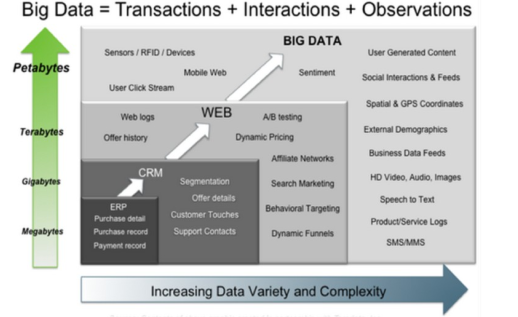
\includegraphics[height=7cm, width=10cm]{../../../images/bigdata.png}
	\caption{Big Data Transactions, Interactions, Observations (Source: \cite{DBLP:journals/corr/MoniruzzamanH13})}
\end{figure}


\[\]


\section{Introduction of NoSQL Databases}

NoSQL, for "Not Only SQL", and as summarized by Moniruzzaman and Akhter Hossain\cite{DBLP:journals/corr/MoniruzzamanH13}, it refers to distributed and non-relational data management systems designed for large-scale data
storage and for massively-parallel data processing across a large number of commodity
servers, where databases are not built primarily on tables and generally do not use SQL for data manipulation. 
NoSQL databases and management systems are schema-less by design. The ability to process massive amount of data with a schema-less structure is also what makes NoSQL more popular in data mining industries where the data that most engineers and data scientists have to work with are  unstructured with flexible schema.
The architecture of NoSQL databases are distributed and fault-tolerant by utilizing replica sets among multiple machine to 
guarantee data availability in the case of network disruption or when certain servers accidentally go down.
To reach a
balance between availability and consistency, NoSQL achieve more optimal
level of consistency by slightly sacrificing its availability.  \\


In a way, RDBMS is still the mainstay in the industry, however, as computational and storage requirements of applications such as for
Big Data Analytics, Business Intelligence and social networking over peta-byte
datasets have pushed SQL-like centralized databases to their limits \cite{DBLP:journals/corr/MoniruzzamanH13}, since it is not built to support distributed system in the first place, the strong focus of relational DBMS on consistency and reliability
and ACID (Atomicity, Consistency, Isolation and
Durability)\cite{neo} guarantee makes it difficult for scaling, which is one of
the many reasons why most companies from giant enterprises to startups are considering migrating their partial or even entire database from RDBMS to NoSQL as business expands. However, NoSQL is not built for the entire replacement of SQL, but as a complementary option for different tasks.
  With sharding, which would be explored in more details later, it partitions data onto a cluster of remote machines, boosting the overall performance while controlling cost with cheap commodity hardware. \\
  
  
\begin{figure}[H]
	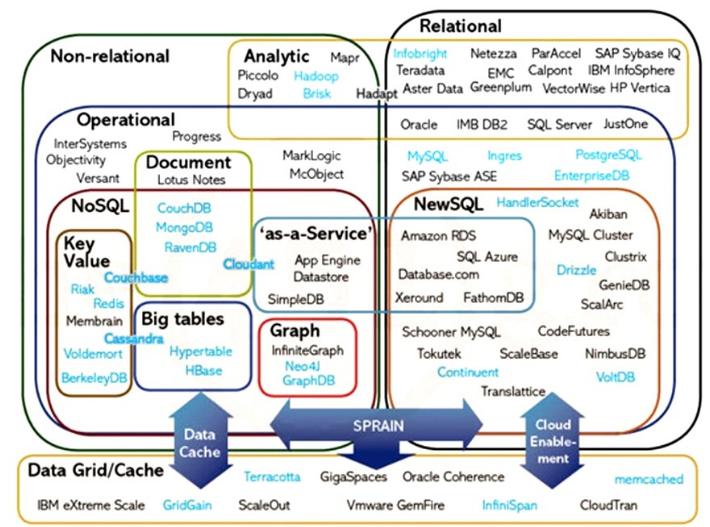
\includegraphics[height=7cm, width=9cm]{../../images/nosql.png}
	\caption{NoSQL Databases in industries (Source: \cite{DBLP:journals/corr/MoniruzzamanH13})}
\end{figure}

  
To take fully advantage of its features such as flexible schema, server failure tolerance and  horizontally scalability by cheap commodity hardware, primary uses of NoSQL Database mainly focus on tasks that requires high velocity of data transaction to guarantee consistency among multiple machines as well as capacity for massive data storage to assure availability. And according to Moniruzzaman and Akhter Hossain\cite{DBLP:journals/corr/MoniruzzamanH13}, these uses include 
\begin{itemize}
\item (1) Large-scale data processing (parallel
 processing over distributed systems); 
 \item (2) Embedded IR (basic machine-to-machine
 information look-up \& retrieval); 
 \item (3) Exploratory analytics on semi-structured data (expert
 level); 
 \item (4) Large volume data storage (unstructured, semi-structured, small-packet structured).
\end{itemize}

\[\]
\section{Characteristics of NoSQL Databases}



\subsection{Availability}

\subsubsection{Replication}\mbox{}

To guarantee high availability, the mechanism of failover is utilized by creating replica sets as remedy for server malfunctions, network disruptions, system maintenance and upgrade. 

\subsection{Scalability}


\subsubsection{Sharding}\mbox{}

In the partitioning step, carefully designed hashing functions are applied to distribute the data as balanced as possible to multiple workers on a cluster to process in parallel. However the improvement of performance comes with sacrifice as well, that across partitions, operations such as joins since the lack of consistency and flexible schema all violate the prerequisite of executing joins. And complex relation features are not supported and referential integrity constraints can also no longer be maintained.


\subsection{Consistency}\mbox{}

As a distributed system, since the writes of data into storage is asynchronous, thus with different architecture, the real-time consistency is not guaranteed, which indicates that clients from different regions are not able to retrieve the same version of data at the same time. But the eventual consistency is absolute after all updates are propagated throughout the system 

\subsubsection{Master-slave}\mbox{}

For databases with master-slave mechanism, all writes into the database are written to the master node, and all reads are processed through the replication set of slave nodes. This centralization architecture could encounter significant inconvenience when the incoming dataset is large, the step when the master node duplicates the data and then passes them down to slave nodes will slow down the entire processing speed. Moreover, if the data written in is somehow incorrect, the mistake would be propogated down to all the slave nodes as well, hence providing the wrong version of data to the users for that the master node is the only source that receives the input raw data.

\subsubsection{Peer-to-peer}\mbox{}

In a peer-to-peer architecture, each node of the cluster is identical to other nodes in a cluster and all nodes follow the dissemination membership protocol and could be considered as request coordinators. Unlike master-slave structure, with peer-to-peer system, the instant consistency could be assured since in the system peers share their resource with other peers and co-ordinate their activities each peer acts both as a client and a server for imparting database services\cite{tutorial}.



\subsection{Summary}
To summarize, since all these three characteristics (Availability, Scalability and Consistency) can not be simultaneously achieved according to CAP theorem \cite{neo}, 

\begin{figure}[H]
	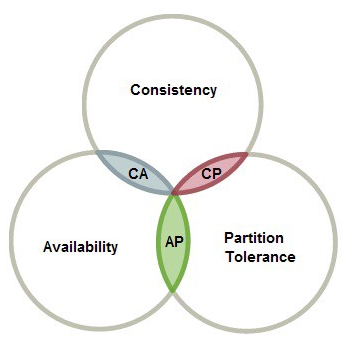
\includegraphics[height=6cm, width=8cm]{../../../images/cap.png}
	\caption{CAP Theorem (Source: \cite{neo})}
\end{figure}

thus compromises are made for trade-offs and balance is reached with the BASE theorem (Basically Available, Soft-state, Eventually consistent)\cite{neo}.

\[\]

\section{Data Models of NoSQL Databases}

An ideal NoSQL model is expected to have the following attributes  high concurrency, low latency, efficient storage, high scalability, high
availability, reduced management and operational costs\cite{DBLP:journals/corr/Sharma15b}. Although various NoSQL databases are currently used in industries depending on the different products and services each company offers to their target clients, there are several major NoSQL in each of its four categories that are most widely used: Redis as key-value store database, Cassandra as column-oriented database, MongoDB as document-oriented database and Neo4j as graph database.

\subsection{Key-Value Databases}

Key-value databases has been around for decades and it's popular among users for its common data structure (key value pair) to store data is easy to understand for java and python programmers because key-value pair shares resemblance with HashMap class in java as well as Dictionary class in python. In key-value databases, keys as field names, are normally represented as unique alpha-numeric identifiers and converted to hashes for more efficient search and retrieve. Correspondingly, the content stored under this field name is its value, which supports various formats of data such as sets, strings and lists. Together, keys and values are stored in standalone hash tables. The performance of key-value databases are mainly affected by:

\begin{itemize}
	\item the design of the hashing function applied to keys. A good hashing function results in fewer conflicts, which ends up with evenly distributed data across all slots;
	\item the size and data format of the corresponding value stored, if the volume of values under each key exceed a certain constraint, then the process of writing into and retrieving from the table could be significantly slowed down, thus compromising the efficiency of the entire task;
\end{itemize}

Since consistency is guaranteed only for operations on a single key, so it would not be an optimal choice for multi-operation transactions or for tasks that involve complex relationship among attributes. However, its simple data structure and compatibility to support multiple data formats assures its outstanding velocity of data processing compared with other  NoSQL databases, thus key-value databases are preferred for caching, user profile managing or shopping cart retrieval. This is why Amazon makes extensive use of its own key value system called Dynamo, a highly available key-value storage
system that provides highly available and scalable
distributed data store in its shopping cart\cite{DBLP:journals/corr/MoniruzzamanH13}. 

\subsubsection{Redis}\mbox{}\mbox{}

As a NoSQL database written in C++, the excel performance and high I/O speed of Redis makes it an optimal choice for 
caching. Redis supports varied data structures such as list, queue, set (basic operations like union, intersection, difference), hash table, stc. 

Redis is preferred for applications with real-time data collecting and processing, which specifically requires high I/O speed because the incoming data is updating rapidly.

\subsection{Column-oriented Databases}

\subsubsection{Cassandra}\mbox{}\mbox{}

Cassandra shines in the applications with large clusters. The replication mechanism guarantees high availability of each data center. And the querying language (CQL) used in Cassandra is quite similar to SQL, hence the learning curve is not as steep as databases like HBase with the entire ecosystem including zookeeper, pig, hive, etc. Rather than the conventional master-slave architecture, Cassandra adopts peer-to-peer distributed
architecture. In Cassandra, each node of the cluster is identical to other nodes in a cluster:

\begin{figure}[H]
	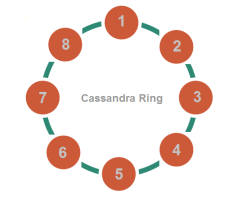
\includegraphics[height=6cm, width=8cm]{../../images/ring.png}
	\caption{Cassandra Ring (Source: \cite{DBLP:journals/corr/abs-1712-04344})}
\end{figure}

 And all nodes follow the dissemination membership protocol and could be considered as request coordinators\cite{DBLP:journals/corr/abs-1712-04344}. 





\subsection{Document-oriented Databases}

Unlike RDBMS designed to store data as tables, Document-oriented Databases are designed to store documents encoded in semi-structured standard data exchange
format such as XML, JSON (Javascript Option Notation) or BSON (Binary JSON)\cite{DBLP:journals/corr/MoniruzzamanH13}.

\begin{figure}[H]
	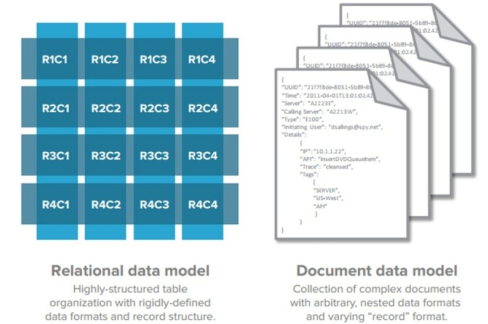
\includegraphics[height=6cm, width=8cm]{../../images/vs.png}
	\caption{Relational data model vs. Document data model (Source: \cite{DBLP:journals/corr/MoniruzzamanH13})}
\end{figure}


 Due to its schema-free feature, under each attribute, multiple nested sub-attributes could be stored in flexible structures that do not have to be identical to each other, which makes Document-oriented databases the perfect option for storing irregular and  sparse data. Because if the amount of missing values is significant in RDBMS, to guarantee a fixed schema structure for the table format, all the missing data would be filled by nulls as placeholders. And in this case, excessive memory would be wasted for unnecessary storage.  


\subsubsection{MongoDB}\mbox{}

Among many NoSQL databases, MongoDB is considered the most popular with the largest number of users. Because not only does it has features of NoSQL database system like flexible schema, easy to scale out and also MongoDB is quite SQL-friendly, for instance, MongoDB allows users to create indexes to speed up the searching process. And the support of writing quries in Javascript and inserting data with a semi-structured format like json, bson, etc. makes MongoDB a user-friendly choice because unlike the other NoSQL databases, it does not require users to learn new syntax specific to the database in order to start using it.


\subsection{Graph Databases}\mbox{}

Graph databases replace relational tables with structured relational graphs of
interconnected key-value pairings\cite{DBLP:journals/corr/MoniruzzamanH13}. Graph theory is applied to the storage of data in graph-based databases, in which each node represents an attribute while each edge represents a relationship between two adjacent nodes, making it nearly as powerful as relational databases when it comes to dataset with complicated relations such as social network. For graph-based databases, it is easy to model all relations that are supported in RDBMS, such as one-to-one, one-to-many and many-to-many because of its hyper-relational feature. But as an improvement compared with relational databases when executing join across multiple tables, graph-based databases aggregate different tables with a much more readable relationship identifier to query data using Depth First Search or Breadth First Search, indicating the fact that it is most suitable for dataset in hierarchical tree structures. Hence it's widely used to map out relationships on social networks and make recommendations for e-commerce platforms.


\subsubsection{Neo4J}\mbox{}

Neo4j is a graph database that is currently under development. With full ACID (Atomicity, Consistency, Isolation and
Durability)\cite{neo} support, it is capable of providing highly availability and stability. It uses Cypher querying language, a declarative language, to execute searching and matching. Both unidirectional and bidirectional relations are supported in Neo4j, which is distinguished by the use of a dotted line in Cypher either with or without an arrow at the end of the line.

\[\]
\section{Benefits And Drawbacks}

\subsection{Benefits}

\subsubsection{Scaling Capability}\mbox{}

The
data size experiences an increase of order of magnitude and in year 2012 alone, it grows from a few dozen
terabytes to many petabytes in a single data set\cite{DBLP:journals/corr/Sharma15b}.
As the rapid expansion and generation of data pushes the conventional RDBMS to its limit, industries are seeking more efficient databases like NoSQL to migrate and storage their data.
Using sharding to partition data onto a cluster of remote machines, NoSQL boosts the overall performance while controlling cost with cheap commodity hardware.


\subsubsection{Flexible schema} \mbox{}

Compared with the conventional RDBMS that any changes of schema must be carefully managed, NoSQL databases has more flexible structure of data and do not need extra adjustments when there are additional requests to update the original schema. 


\subsubsection{Cost}\mbox{}

One outstanding feature that makes NoSQL a widely used database among various industries with massive amount of data manipulation involved is that it takes advantage of clusters of cheap commodity servers for data storage and transaction.
Compared with expensive propriety servers that RDBMS used to rely on, cost per transaction using NoSQL is lower, so NoSQL is considered much more economically preferable.  


\subsubsection{Summary}\mbox{}

According to the results of a Couchbase Survey conducted in the 2012,  NoSQL has moved beyond the experimentation phase moving in deeper ways to meet the data management requirements of their applications\cite{drive}.

\begin{figure}[H]
	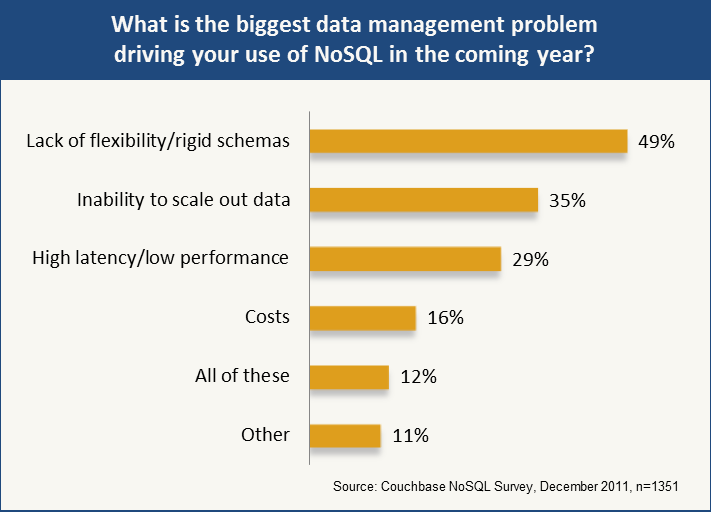
\includegraphics[height=7cm, width=8cm]{../../images/drive.png}
	\caption{Biggest data issues motivate driving to NoSQL (Source: \cite{drive})}
\end{figure}

\subsection{Drawbacks}

However there are still many remaining problems which NoSQL
databases cannot solve:

\subsubsection{Not Support Complicated transactions}\mbox{}

Since NoSQL is specifically built for distributed data management, hence its non-ACID reliant  and schema-free  feature  does not guarantee the absolute consistency (only assure eventual consistency) and homogeneous data structure. So when it comes to complex relationships or transactions between attributes, NoSQL would not be capable to support such operations:
\begin{itemize}
	\item Join
	\item Aggregate
\end{itemize}

\subsubsection{Standardization}\mbox{}

Unlike RDBMS, the wide variety of design and query languages of NoSQL databases between different NoSQL products entails a much steeper learning curve for NoSQL databases, which makes it a barrier to NoSQL adoption for organizations keen to maximize the usefulness of staff expertise\cite{limit}.


\subsubsection{Reputation}\mbox{}

Though NoSQL data
models are rapidly developing and become more and more popular among DBAs, RDBMS still has a larger market and well-established reputation than NoSQL, most of which are open source projects with support from startups, the client support of RDBMS is more mature. 
The reason
is that the NoSQL data models are still alien for most of the organizations who
neither feel knowledgeable nor confident enough to rightly decide about which of the NoSQL data model
may better serve their need\cite{DBLP:journals/corr/Sharma15b}.

\begin{figure}[H]
	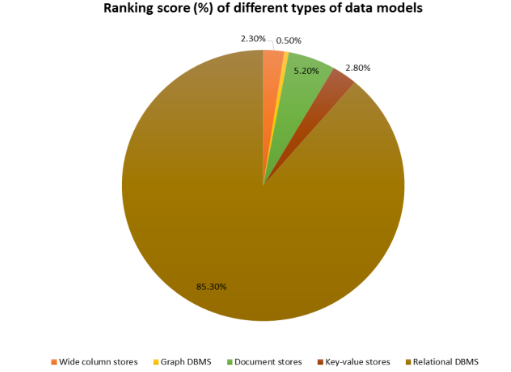
\includegraphics[height=7cm, width=9cm]{../../images/rank.png}
	\caption{Ranking score of different types of data models (Source: \cite{DBLP:journals/corr/Sharma15b})}
\end{figure}


\subsubsection{Security}\mbox{}

Currently under active development,
NoSQL databases are generally subject to a fairly long list of security issues such as weak password storage, lack of encryption support for the data files, weak authentication both between client and the servers, data at rest is unencrypted, etc \cite{deka2014handbook}.

\[\]

\section{Conclusions}

Nowadays, the exponential usage of digital devices and massive data generation that comes after post both great opportunities and also unprecedented challenges to all data managing enterprises, startups, institution as well as data scientists and engineers.
The demand to scale out in order to store and process the accumulating data is a urgent problem as business expands and the client pool enlarges. That's when NoSQL comes into play. This paper gives a precise introduction of the  features (Availability, Scalability and Consistency) of NoSQL DBMS and provides comparisons among some of the most widely used NoSQL databases from their architectures, data models and suitable applications and scenarios. The classification (key-value store, column-oriented store, document-oriented store and graph-based store) and the most prominent representatives of each are also discussed. The benefits and drawbacks illustrated is aimed to help both academic and industrial users to have a more thorough understanding of NoSQL databases before deciding which one or ones to use for their own tasks. NoSQL as a promising substitute for the conventional relational database system, presents its unparalleled advantages especially when manipulating amount of data up to petabytes or terabytes and unstructured sparse data, which makes the comparison and evaluation among popular NoSQL database systems in analyzing big data a potential subject in future work that is worth further exploration. 

\[\]
